%
% File acl20ying a ontact: Maggie Li (cswjli@comp.polyu.edu.hk), Michael White (mwhite@ling.osu.edu)
%%
%% Based on the style files for ACL2008 by Joakim Nivre and Noah Smith
%% and that of ACL2010 by Jing-Shin Chang and Philipp Koehn
\documentclass[10pt,a5paper,twoside]{article}
\usepackage{coling2012}
\usepackage{amsmath}
\usepackage{url}
\usepackage{subfig}

\title{Detecting English Writing Styles For Non Native Speakers}

\author{$Rami~Al-Rfou'~~~Yejin~Choi$ \\
  Department of Computer Science \\
  Stony Brook University \\
  NY 11794, USA \\
  \texttt{ \{ralrfou, ychoi\}@cs.stonybrook.edu}}


\begin{document}
\maketitle
\abstractEn{
This paper presents the first attempt (up to our knowledge) to classify English
writing styles on this wide scale. The corpus that is extracted from Wikipedia
represents a day to
day language written by authors with different backgrounds and skills covering
various categories of topics. To solve such hard problem, we propose simple
machine learning algorithms and easy to generate features.
The scale of the data available from large sources of knowledge like Wikipedia
makes it possible to generate robust solutions for the web with high accuracy
and easy to deploy in practice.
The paper achieves 74\% accuracy classifying native versus non native speakers
writing styles and offers a publicly accessible corpus for further studies of
various writing styles. Moreover, this paper makes interesting observations on the similarity between
different languages measured by the similarity of their users' writing styles.
This technique can be used to show some well known linguistic theories about
languages, as in grouping them into families according to their origins and
development history.}

%TODO
\keywordsEn{bla, bla}

\newpage

\section{Introduction}
With the introduction of social networks and media, the content on the internet 
has become more diverse than ever and the distribution of users has changed.
Learning languages and improving the fluency of non native speakers has
become more important. Since English is the universal language of communication, we chose the English
non native speakers to understand the influence of their
native languages on their English writing styles.

We believe the task of identifying the user's native language serves an essential
step to advance the state of art of the applications in the areas of misspelling and grammatical errors
correction, paraphrasing and speech recognition.

Wikipedia is a well known source of knowledge. Recently, it is has been used extensively
to help solving different information retrieval tasks, especially the ones
that involves semantic aspects\cite{Milne08aneffective}. The use of Wikipedia can be expanded to help the
common NLP tools to perform better; the size of the data and the diversity of
authors and topics plays a key role. Moreover, the sustained growth of Wikipedia
content of can bring performance gains with no much additional complexity costs.

This paper is structured as follows. In section \ref{rwork} we discuss the
literature of identifying users' native languages from their English writing
styles. Section \ref{wiki} discusses various aspects of Wikipedia content and
the methodology used to generate the corpus used in the following experiments.
Section \ref{exps} describes the setup of the experiments conducted on the
Wikipedia extracted corpus and the results of each. In section \ref{conc} we
give conclusions regarding the presented results and comments on possible future
work aspects.


\section{Related Work}
\label{rwork}
The first work related with native language identification is that of
\cite{koppel2005automatically}, in which they tried profiling anonymous authors
with their native languages. Five groups of non native speakers; Russian,
Bulgarian, Czech, French, and Spanish were picked from the first version of {\em
International Corpus of Learner English} (ICLE). By applying a combined feature
sets, including function words, character n-grams, part-of-speech bi-grams and
spelling mistakes, they gained an accuracy of 65\% if considered style features
only. These results suggested that syntactic features are valuable when trying
to categorize authors by their native languages. Also in \cite{koppel2005determining},
they considered not only letter n-grams and function
words but errors and idiosyncrasies, including orthography errors, syntax
errors, neologisms and part-of-speech bigrams errors. Finally the accuracy on
classifying authors with the five different native languages can reach above 80\%.
\cite{argamon2009automatically} concluded some more important features in the task of profiling authors of an anonymous text.

Similar work has been done by \cite{tsur2007using}. They focused on the
relationships between choice of words in second language writing and the
frequency of native language syllables, also known as the phonology of native
languages. \cite{estival2007author} studied a wide range of lexical and
document structure features in their native languages classification task. And
\cite {zheng2003authorship}, though they did not directly conduct related
experiments on nationality detection, they provided some features of style marks
that could be used in the task of judging one's native language. Besides, \cite {gamon2004linguistic}
analyzed the power of some general features under
different frequency cutoffs. However, none of these measured the usefulness of
syntactic features under a general condition for the task of native language
detection.

\cite{wong2009contrastive} replicated the work of \cite {koppel2005automatically}
and dug more in the field of syntactic structures.
They experimented on three selected syntactic errors, which are commonly
observed in non native English users, including subject-verb disagreement,
mismatch of noun-number pairs and wrong usage of determiners and the best
overall accuracy was 73.71\% on the second version of ICLE across seven
languages. \cite{wong2010parser} first considered applying parser features in
the task though these features are hard to extract compared with other
syntactic features. In \cite{wong-dras:2011:EMNLP}, they continued their
work in native language detection and focused more on the influence of
syntactic structures, specifically parsing trees. They tried to exploiting the
parsing structures by applying Standford parser and C\&J parsers with different
parameters to certain corpus, and capture the frequent patterns of usage of some
distinguishable rules. Their results and observations suggested that the
syntactic structures would be supportive in detecting native languages and
improving the performance of existing classifiers.

Different from the previous works mentioned above, our task targets totally
different corpus, Wikipedia. Wikipedia represents more challenging content as the
authors are more technically advanced in their language skills since it is not only written by
new learners of English. Moreover, most of the contributions to Wikipedia are
small in size, either by modifying a developing article or commenting on
a mature one. Our goal here, is to find out the influence of one's native
languages on the style of his/her writings under the circumstance of talking and
discussion.

\section{Wikipedia}
\label{wiki}
Wikipedia is the de facto source of knowledge for internet users. Wikipedia is
the 6\textsuperscript{th} most popular website according to Alexa ranking.
For researchers Wikipedia is a giant linguistic and social jar of experiments.
The richness of the website content that is written by users from different backgrounds represents a robust sample of the current languages usage by native and non native speakers.

With more than 90 thousand active users and 4.4 million article, the content of Wikipedia spans large number of topics. The diversity of authors beside the records of versions that are stored in a database of revisions presents a realistic source of text. Such resource presents a higher quality of data that is not achievable by the other commonly used sources of text as news, blogs and scientific articles.

Such successful website has a complex database structure to serve its users.
Therefore, extracting data is a complex process. Our goal is to identify the
languages skills of the users and collect their contributions. To achieve the
first task Wikipedia has an information box called \emph{Babel} that users can
add voluntarily to their profile pages to state their skills in different
languages. Figure \ref{babel} shows a user who identified her native language
and her skills in 3 other non native languages on a scale of 0-5. This info box
is indexed in the database as a category.

\begin{figure}
\centering
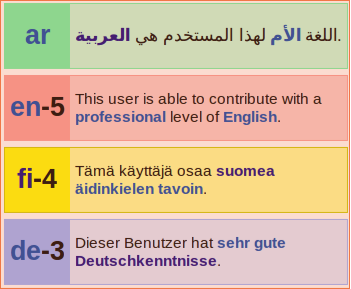
\includegraphics[scale=0.40]{babel} 
\caption{Wikipedia languages skills info box (Babel)}
\label{babel}
\end{figure}

The task of collecting the contributions of a specific user is more complex
procedure. The diffs between Wikipedia pages revisions has to be generated and
linked back to the user table. The resources we have are not sufficient enough to process such
huge amount of data\footnote{Recent efforts were
made to generate the diffs \url{http://dumps.wikimedia.org/other/diffdb/}}.
Instead we noticed that Wikipedia pages have accompanying discussion pages where
users discuss different aspects of the articles. In those pages the tradition is
that the user will sign his own comments with a signature that link back to the
user page. Figure \ref{obama} shows an example of those comments. The style of writing of those
talk pages are less formal and technical than the main pages of Wikipedia and has more conversational stylistic features.

\begin{figure*}
\centering
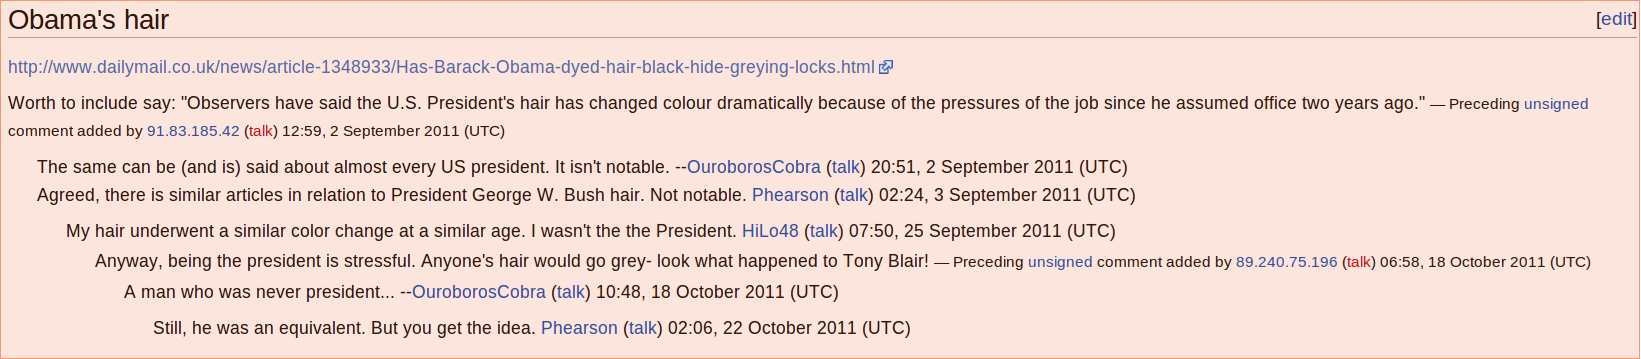
\includegraphics[scale=0.225]{obama.png}
\caption{Example of a conversation in the discussion pages}
\label{obama}
\end{figure*}

The recommended signatures patters are limited, however, in practice the users
use various patterns that makes the detection rules ambiguous. The detection
algorithm that we implemented relies on complex regular expressions and applies best effort strategy.

\section{Experiments}
\label{exps}
We found that around 60 thousands users specified their language skills. Figure \ref{native_dist} shows that the percentage of users who claimed that their native language is English is around 47\% of English Wikipedia users base.

\begin{figure}
  \centering
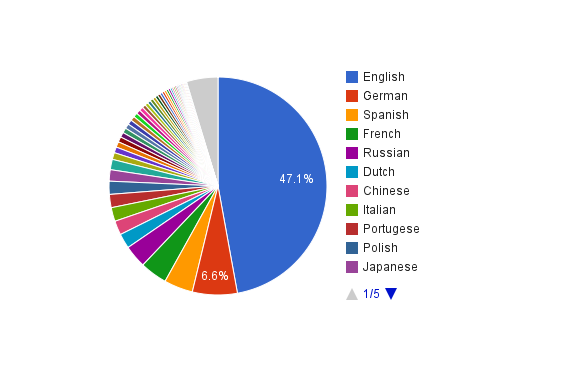
\includegraphics[scale=0.36]{chart_4.png}
\caption{Users distribution over native languages in English Wikipedia}
\label{native_dist}
\end{figure}

We parsed the talk pages with the \verb+namespace=1+, they represent more than
80\% of the talk pages. The total number of comments found in those pages is
around 12 million comment. Only 2.4 million comment has users with identified language skills. As not all the users contributes to the talk pages, the number of users who makes at least one comment in the extracted comments is around 30 thousand user.

Since we have large number of comments and users, we can apply more filtering to
increase the quality of the data gathered. Therefore, we applied the following filtering mechanisms:
\begin{compactitem}
\item Users are grouped according to their native languages. Users of the most frequent 20 native languages are selected.
\item English native speakers can identify more information by specifying which
variation of English they are familiar with. Only US English native speakers are
selected. This decision was made to avoid the variations of standard English
among different dialects and countries. Moreover, this step helps us to filter
the non native speakers who are proficient in English so they choose the general
Native English category in their skills instead of specifying their skill to be
at level 5.
\item Users who specified more than one native language are excluded. This step
helps us to avoid improbable scenarios where users claim to be native in many
languages.
\end{compactitem}

The new data set after the filtering is composed of 9857 user and 589228 comments.

\subsection{Setup}
The following experiments are conducted under the following conditions:
\begin{compactitem}
\item The accepted comments have to have at least 20 tokens.
\item Proper nouns are replaced by their tags to avoid bias toward topics.
\item Non ASCII characters are replaced by a special character to avoid bias toward non English characters usage in the comments.
\item The classifier has balanced number of comments for each of its classes. Therefore, the two baseline classifiers; the most common label and the random classifier will have an accuracy of \verb+1/number of classes+.
\item The data set is split to 70\% training set, 10\% development set and 20\%
as a testing set.
\end{compactitem}

\subsection{Features}
The comments of the training set is grouped by class and the following frequency distributions are calculated for each class:
\begin{compactitem}
\item 1-4 grams over the comments' words.
\item 1-4 grams over the comments' characters.
\item 1-4 grams over the part of speech tags.
\end{compactitem}

For each comment ($C$), similarity measurements ($Sim$) are calculated against each \verb+n-gram+ frequency distribution ($f(n)$) according to the following equations:

\[
  count(x, f, n) = \left\{ 
  \begin{array}{l l}
    FreqDistCount(x, f, n), & \\\quad \text{if $x$ is in $f(n)$}\\
    1,&\\\quad \text{if $x$ is not seen before}\\
  \end{array} \right.
\]
\[
  Sim(C,f,n) = \sum_{x \in ngrams(C,n)} \log_2 (count(x,f,n))
\]

Therefore, if the problem has six classes, this will generate $6*3*4 = 72$ features.

Other features also includes the relative frequency of each of the stop words to
the size of the comments. The 125 stop words are extracted from the NLTK stop
words corpus\cite{nltk}. Moreover, the average size of words, the size of the comments and the average number of sentences are also included.


\subsection{Native vs Non Native Experiment}
This experiment aims to detect the non native speakers comments. All users with native language other than English are placed into the same category. The number of comments used is around 322K comment. Table \ref{table:results} shows that the linear SVM classifier succeeds to reach $74.53\%$ accuracy. Figure \ref{non_cfm} shows the confusion matrix of the classifier.


\begin{figure}
\centering
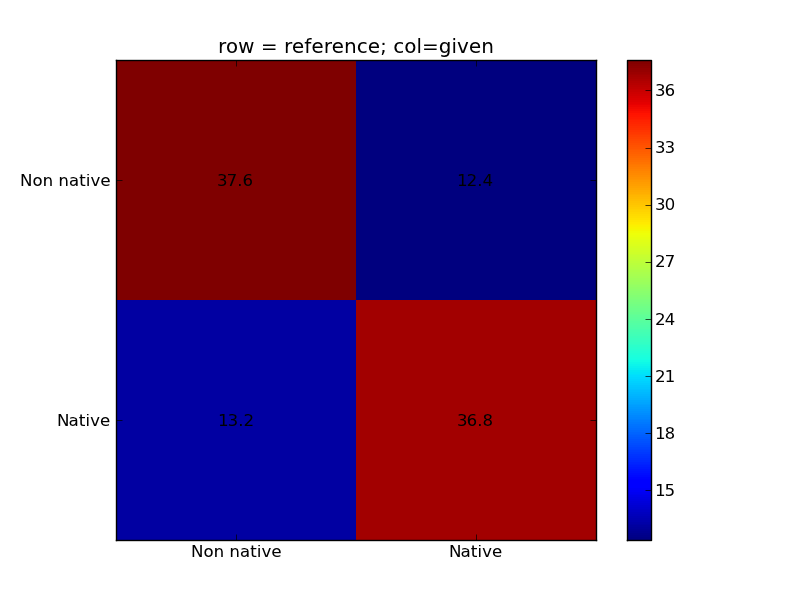
\includegraphics[scale=0.35]{native_cfm.png}
\caption{Native vs Non Native speakers experiment confusion matrix}
\label{non_cfm}
\end{figure}


The most informative features are words trigrams, words uni-gram, words bi-gram, words 4-gram, characters bigrams, PoS tags 4-grams, ordered by their importance. Table \ref{table:nonnative} shows the most correlated grams with native languages.

Some of the grams indicate possible common grammatical mistakes in the Non native speakers writing styles. Unigrams over words shows that non native speakers tend to use earth instead of Earth. Characters bigram shows that separating the comma from the previous word by a space is common usage of punctuation for non native speakers.
The usage of articles is a problematic issue for non native speakers, in the words 4-grams we can see using the article \emph{the} before a proper noun is a frequent pattern, this trend of using \emph{the} more than needed can be confirmed by the characters bigrams where \emph{th} appears. Word trigram shows that native speakers use \emph{the} correctly in \emph{in the middle} where we expect non native speakers to use \emph{in middle}.
Moreover, from the characters bigrams non native speakers use \emph{at} less than the native speakers which could suggest that they misuse the other articles where \emph{at} should be used. Characters bigrams shows a trend in spelling mistakes, where non native speakers type single \emph{l} instead of \emph{ll}. Another spelling usage trend is the less frequent usage of apostrophes \emph{'}, this can be traced by the more frequent usage of \emph{am} in words unigrams for non native speakers and the appearance of \emph{don't} in the words 4-grams for native speakers.

\begin{table}[t]
\begin{center}
\subfloat[Correlated grams and native languages for detecting non native speakers experiment]{
\begin{tabular}{l|ll}
	\textbf{Feature} & \textbf{Speaker}  & \textbf{Gram}
	\\\hline
	Words & Non Native &article on NNP\\
      Trigrams& &  \emph{comma} you have\\
	 & Native& used in the\\
	 &  &in the middle\\\hline
	 
	Words &Non Native& scene, To,\\
	   Unigrams&&describing, earth,\\
	    && referenced, am\\\hline
	    
	Words 	&Non Native& You have, we do\\
	Bigrams&& of people\\
	&Native& years of, I see\\
	&&if you\\\hline

	Words &Non Native& but I think that\\
	4-grams	&&by the NNP of\\
		&&( or at least\\
		&Native&NNP on NNP NNP\\
		&&if you don't\\\hline

        Characters&Non Native& th, e \emph{space},\\
          Bigrams && \emph{space} \emph{comma}\\
	&Native& l-, at, ll\\\hline
	
	PoS 4-gram &Non Native& NNS \textbf{,} DT NN\\
	&& MD VB VBN \textbf{,}\\
	&Native& \textbf{,} PRP VBZ JJ\\
	&& VBP NN IN NN\\
      \end{tabular}
    \label{table:nonnative}}
\subfloat[Correlated grams and speakers for the most frequent languages experiment]{
  \begin{tabular}{l|ll}
	\textbf{Feature} & \textbf{Speaker}  & \textbf{Gram}
	\\\hline
	Words & Russian &prove that\\
	 Bigrams& German& you leave\\
	 & Spanish& to reveal\\
	 & Dutch & reliance on\\\hline
	 
	Words &Dutch& refuting\\
	   Unigrams&Spanish&timelines\\
	    &German& tie\\\hline
	    
	Words 	&Russian& stick to what\\
	Trigrams&Spanish& find out the\\
	&Dutch& end up in\\\hline

        Characters &French& hee \emph{space}\\
	4-grams	&French&ownr\\
		&Dutch&c/es\\
	\hline

	Words &French& NNP as far as\\
	4-grams &German& the NNP who\\
	&Spanish& ,etc),\\
	&EN-US& Does anyone know if\\\hline
	
	PoS 4-gram &Dutch& RB CD -RRB- IN \\
	&EN-US& VBD , RB DT\\
	&EN-US& CD VBD NNS IN\\
	&& \\
	&& \\
	&& \\
\end{tabular}
\label{table:nonnative}}
\end{center}
\end{table}

The more fluent the speaker is in English the closer his/her writing
style to the native speaker style. To test our basic intuition,
we have to take advantage of the specific language fluency levels that the speaker can choose
from the available Wikipedia Babel box categories. We designed two different
variations of the previous experiment. In the first we limited
the non native speakers category to the speakers with basic skills in English,
those who correspond to \verb+User_en-0+ to \verb+User_en-2+ of Wikipedia categories.
While the second is composed of the more advanced non native speakers with
English levels ranging from \verb+User_en-3+ to \verb+User_en-5+.
Figure \ref{fluency} shows the classifier error rate in the three previous
variations.

\begin{figure}
\centering
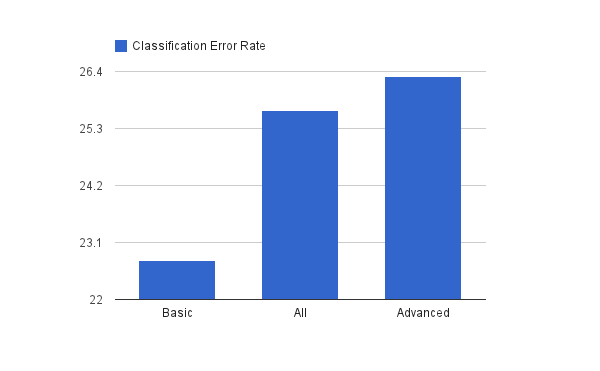
\includegraphics[scale=0.50]{fluency.png}
\caption{Classification error rate against non native speakers with different
skills.}
\label{fluency}
\end{figure}

The increase of the error rate of classification confirms our intuition.
Moreover, it increases our confidence in the information the users mention in
their profiles regarding their language skills.

\subsection{Frequent Languages Experiment}
This experiment aims to classify the comments written by the speakers of the most frequent native languages.
Six languages are selected US-EN, German, Spanish, French, Russian and Dutch.
Figure \ref{pop_cfm} shows the confusion matrix of the logistic regression
classifier. The data set size is about 150K comment. We can see clearly that the
Russian users are the easiest to identify. Moreover, the classifier is the most
confused distinguishing the German and the Dutch users with error $>2.0\%$ and
to a less degree between (EN-US, French). These numbers confirm a basic
intuition that the languages that have geographical proximity will have more
borrowed words and grammars between them. And accordingly this will affect their speakers writing styles in English.

\begin{figure}
\centering
\subfloat[Frequent languages experiment confusion matrix]{\label{pop_cfm}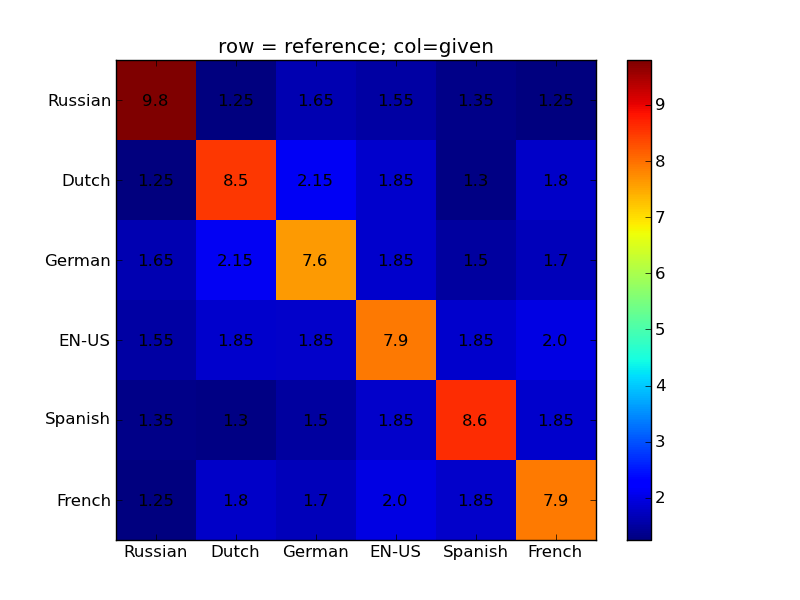
\includegraphics[scale=0.35]{popular_cfm.png}}
\subfloat[Languages families experiment confusion matrix]{\label{fam_cfm}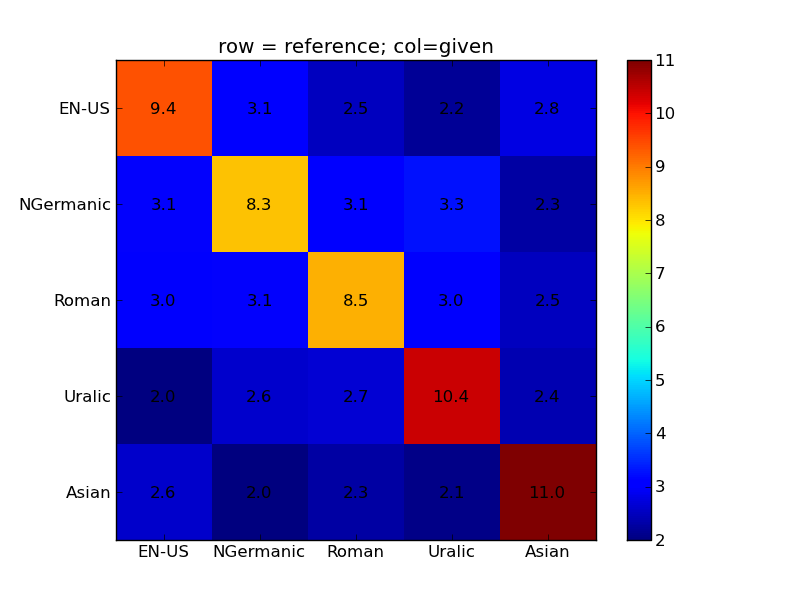
\includegraphics[scale=0.35]{family_cfm.png}}
\end{figure}

The most informative features are ordered as the following, words bigrams, words
unigrams, words trigrams, characters 4 grams, words 4 grams, PoS tags 4-grams.
We can see that the features of the longer grams become less informative once we
increased the number of classes given to the classifier. The increasing
importance of shorter grams of words may indicate the influence of the topic of the comment on the classification.

Table \ref{table:results} shows that the best accuracy that the classifier achieved is 50.27\% with 77K comment used. 
\subsection{Languages Families Experiment}

The confusion in classifying Dutch and German users suggests that there is a similarity between groups of languages. Referring to the linguistics research history of classifying the languages into families according to similar features and development history, this experiment tries to put such grouping under the microscope. 18 languages are grouped into 5 families as the following:
\begin{compactitem}
\item \textbf{Germanic}: German, Dutch, Norwegian, Swedish, Danish.
\item \textbf{Romanace}: Spanish, French, Portuguese, Italian.
\item \textbf{Uralic}: Finnish, Hungarian.
\item \textbf{Asian}: Mandarin, Cantonese, Japanese, Korean.
\item \textbf{Slavic}: Russian, Polish
\end{compactitem}

Figure \ref{fam_cfm} shows the that the Slavic and Asian native speakers has a clear style of writing English that is easy to detect relatively. The highest confusion in classification is between the Germanic and Romance languages, where geographical proximity plays a role in similarity. With the same reasoning we can see the confusion between Germanic and Uralic languages.


Taking the opposite approach, we took the speakers of the most frequent 20
native languages and applied the same classification procedure over the new
classes. The accuracy of the classifier is 25\%. However, considering the
confusion matrix as a similarity matrix, we applied the affinity propagation
clustering algorithm\cite{sklearn} over the confusion matrix and the clusters that are formed are the following:
\begin{compactitem}
\item \textbf{Cluster 1}: Arabic.
\item \textbf{Cluster 2}: Danish, Dutch, Finnish, Norwegian, Swedish.
\item \textbf{Cluster 3}: French, Italian, Portuguese, Spanish.
\item \textbf{Cluster 4}: Mandarin, Cantonese, Japanese, Korean.
\item \textbf{Cluster 5}: Russian, Polish, Turkish.
\item \textbf{Cluster 6}: Hungarian, German, US-EN.
\end{compactitem}

The above clusters support to large extent the literature classification of
languages. Scrutinizing the 4-grams POS tags reveals more interesting
observations regarding non native speakers usages for English. For example,
in Portuguese speakers comments the pattern \verb+IN DT NN PRP+ appears 0.13\%
of the total number of their comments POS 4-grams. However, it only appears
0.04\% in the Korean speakers comments. Another notice can be detected by
looking at the \verb+NN NN IN DT+'s usage in Portuguese and Polish comments. It
appears 0.15\% in the former POS 4-grams but only 0.05\% in the later. Arabic
speakers tend to use the pattern \verb+TO DT NN IN+ so frequently that it
appears 0.11\% while it is less than 0.06\% for other speakers POS 4-gram
distributions. Finally, Japanese and Danish speakers slightly prefer the pattern
\verb+NN PRP VBZ RB+ more than others.

\subsection{Learning Algorithms}

Table \ref{table:results} shows negligible differences between different learning algorithms used in the experiments. 

\begin{table}
  \begin{center}
  \begin{tabular}{l|ll}
	Experiment & Logistic Regression & Linear SVM
	\\\hline
	Non Native & 74.45\% & 74.53\%\\
	Frequent & 50.27\% & 50.26\%\\
	Families & 50.81\% &50.53\% \\
\end{tabular}
\caption{Accuracy of classification using different learning algorithms.}
\label{table:results}
\end{center}
\end{table}

Figure \ref{comb_lc} shows a typical over fitting situation where the more data
you have the better the classifier can achieve. And here the size of data that
can be extracted from Wikipedia plays a significant role to boosts the accuracy
from 37\% to over 50\% in case of the Frequent languages and Families of
languages experiments. This confirms the importance of the coverage of words in
the language models that supplies the frequency counts on the performance of the classifier.

\begin{figure}[t]
\centering
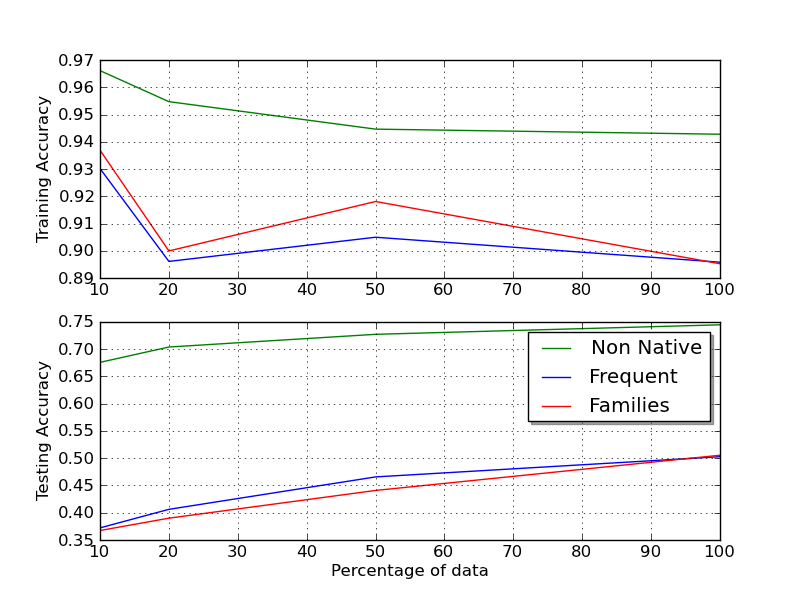
\includegraphics[scale=0.45]{combined_lc.png}
\caption{Learning curves of the logistic regression algorithm.}
\label{comb_lc}
\end{figure}


\section*{Conclusions and Future Work}
\label{conc}
As our results shows promising applications and trends using Wikipedia data to solve hard problems in robust means, there are many paths to improve our results and discover more interesting insights.

Moreover, as the learning curves show, it worth the effort increasing the size
of the data in order of magnitude by adding the Wikipedia diffs, especially the
non minor ones, as it represents another source of users' contributions. Moreover, the minimum size of the comments affects the performance of our classifiers, the relation between the quality of the data used and the accuracy of the classification is another interesting aspect.

The languages families experiments suggest the usefulness of using the English writing styles to define the similarities between different languages. This could lead to an interesting explanations and/or observations regarding the origins of some languages as Korean language which still a controversial topic.

Another direction is to solve the over fitting problem in our learning algorithms by applying smarter feature selection and adding more distinguishing features.

\section*{Acknowledgements}
We would like to thank Steven Skiena for the discussion and the advice. This
work will not be available without the computing resources offered by his lab.
We are also indebted to the NLTK and the Sklearn teams for producing excellent
NLP and machine learning software libraries.

\bibliography{myrefs}{}
\bibliographystyle{apa}

\end{document}
